\section{Ejercicio 5}
\subsection{Introducción}
\noindent El objetivo de este ejercicio es resolver nuevamente el problema de MCS, pero esta vez con una heurística de búsqueda local, ya que suponemos que resolver el problema de forma exacta no se puede hacer en tiempo polinomial, pero sí podemos implementar un algoritmo heurístico que se ejecute eficientemente (tiempo polinomial) aunque no garantice la solución optima.
\subsection{Heurística}
\noindent Esta heurística se basa en moverse de una solución a otra solución vecina, es decir, a una solución similar a la anterior. Para ello es necesario determinar una función de vecindad para que dada una solución inicial, se la pueda modificar levemente dependiendo de algún criterio para obtener una nueva solución que supere a la anterior. Luego se repite este proceso hasta que no exista vecino de la solución actual que la supere.\\
El problema de este método es que se mueve a otra solución sólo si ésta es mejor que la anterior. Muchas veces sucede que para llegar a la solución óptima desde el resultado de partida es necesario pasar por algún resultado intermedio que genere menos aristas en el subgrafo común que el mejor obtenido hasta el momento. Como esta heurística no se mueve a soluciones intermedias peores puede pasar que el resultado no sea el óptimo real si no que sea un óptimo local, es decir, una solución óptima en una rama de soluciones cuando la mejor solución se encuentra en otro lado.

\subsubsection*{Vecindades}
\noindent En este ejercicio se analizarán dos criterios distintos para determinar cuando una solución es vecina de otra.
El algoritmo recibe dos grafos y se quiere hallar al máximo común subgrafo entre ellos. Sea $G1$ el que tiene la menor cantidad de nodos y $G2$ el otro. Si ambos tienen igual cantidad de nodos es indistinto cuál es $G1$ y cuál es $G2$.\\
Sea el vector mapeo el mismo que en el ejercicio 2.\\
\noindent Luego, dado un mapeo, se busca cuál es el conjunto de aristas que tienen en común ambos grafos renombrando cada nodo $i$ de $G1$ como $mapeo[i]$, es decir, el nodo que antes era el nodo $i$ ahora se llamará $mapeo[i]$.\\
Lo que queremos hallar es el mapeo para el cual la cantidad de aristas comunes entre los grafos sea la máxima posible ya que se sabe que la cantidad de nodos del máximo subgrafo común coincide con la cantidad de nodos de $G1$. \\

\noindent Sea $mapeo$ el vector de mapeo al que se le quiere buscar los vecinos y $mapeoVecino$ un vector de mapeo vecino de mapeo.


\subsubsection*{Vecindad tipo 1}
\noindent Dado un mapeo, un mapeo vecino válido es aquel que cumple con alguna de las siguientes condiciones:
\begin{itemize}
	\item Es igual que $mapeo$ pero tiene únicamente dos posiciones intercambiadas ($mapeoVecino[i] = mapeo[j]$ y $mapeoVecino[j] = mapeo[i]$ con $i \neq j$).
    \item Para alguna posición del vector mapeo se modifica el valor por otro que corresponde a un nodo de $G2$ que no estaba siendo utilizado en el vector anterior ($mapeoVecino[i]$ = $j$, con $ 0 \leq j$ $<$ $cantidad$ $de$ $nodos$ $de$ $G2$  y $j$ $\neq$ $mapeo[k]$ $\forall$ $0 \leq k <$ $cantidad$ $de$ $nodos$ $de$ $G1$).
\end{itemize}
\subsubsection*{Vecindad tipo 2}
\noindent Dado un mapeo, un mapeo vecino válido es aquel que cumple con alguna de las siguientes condiciones:
\begin{itemize}
	\item Es igual que $mapeo$ pero tiene únicamente tres posiciones intercambiadas ($mapeoVecino[i] = mapeo[j]$, $mapeoVecino[j] = mapeo[k]$ y $mapeoVecino[k] = mapeo[i]$, con $i \neq j \neq k$).
    \item Para alguna posición del vector mapeo se modifica el valor por otro que corresponde a un nodo de $G2$ que no estaba siendo utilizado en el vector anterior ($mapeoVecino[i]$ = $j$, con $ 0 \leq j$ $<$ $cantidad$ $de$ $nodos$ $de$ $G2$  y $j$ $\neq$ $mapeo[k]$ $\forall$ $0 \leq k <$ $cantidad$ $de$ $nodos$ $de$ $G1$).  
\end{itemize}

\subsection{Implementación}
\begin{algoritmo}{MCSbusquedaLocalUno}{vector(int) mapeo, vector(vector(int)) grafoChico, vector(vector(int)) grafoGrande}{vector(int)}

	\tipo{vector(vector(int))} vecindadA = calcularVecindadTipoA(mapeo);\com*{En vecindadA se tiene el conjunto de mapeos vecinos a mapeo que cumplen con el primer criterio de alguna de las vecindades mencionado en la sección vecindades} 
    \tipo{vector(vector(int))} vecindadB = calcularVecindadTipoB(mapeo, grafoGrande.size());\com*{En vecindadB se tiene el conjunto de mapeos vecinos a mapeo que cumplen con el segundo criterio de alguna de las vecindades mencionado en la sección vecindades} 
    \tipo{vector(int)} mapeoNuevo = dameElMejorVecinoDelMapeoActual(vecindadA, vecindadB, mapeo, grafoChico, grafoGrande);\com*{En mapeoNuevo tengo el mejor mapeo vecino al mepeo actual} 
     
     \While{ExisteVecinoDeLaSolucionActualQueLaSupere(mapeo)}{
		mapeoNuevo = dameElMejorVecinoDelMapeoActualOMejorActual(vecindadA, vecindadB, mapeo, grafoChico, grafoGrande);	\com*{Devuelve el mejor entre todas los los mapeos vecinos. En caso de que no haya uno mejor devuelve el mapeo actual} 
        \If{(noSonIguales(mapeo, mapeoNuevo))}{
       		mapeo = mapeoNuevo
        	vecindadA = calcularVecindadDosTipoA(mapeo);
			vecindadB = calcularVecindadTipoB(mapeo, grafoGrande.size());
      	}
  }
        
\end{algoritmo}
\subsubsection*{Correctitud}
\noindent Veamos ahora que el resultado final es un subgrafo. El grafo inicial es subgrafo ya que iniciamos con un mapeo que devuelve el algoritmo de heurística golosa y, como demostramos antes, es un mapeo que genera un subgrafo válido. Luego lo que hace la heurística es moverse a una solución vecina, lo que genera un nuevo mapeo. Veamos ahora que para cualquiera de las vecindades este mapeo sigue siendo válido: 
\begin{itemize}
	\item Cuando sólo cambio dos o tres de lugar el mapeo no puede pasar a ser inválido ya que todos los nodos de $G1$ siguen estando mapeados con otros nodos de $G2$, lo único que se cambió fue con qué nodo se encuentra mapeado cada uno de los que se modificó.
    \item Cuando se cambia el valor de uno por otro que no estaba siendo utilizado, sigue siendo un mapeo válido ya que para todos los nodos que no se modificó el mapeo sigue siendo lo mismo, y el nodo modificado está mapeado con uno que no estaba siendo utilizado y que pertenece a los nodos de $G2$. Entonces el mapeo sigue siendo válido. 
\end{itemize}
Entonces cuando busco los vecinos de un mapeo aplicando cualquiera de las dos vecindades vuelvo a obtener un mapeo válido. Si vuelvo a aplicar tantas veces como sea necesario hasta que no exista vecino de la solución actual que la supere, como cada vez que lo aplico parto de un mapeo válido (porque, o es la primera vez que parto del goloso o es el resultado de aplicarle a un mapeo válido la vecindad) entonces el mapeo final es un mapeo válido. \\
Luego lo que se hace con este mapeo es buscar las aristas que tienen en común ambos grafos, por lo tanto la respuesta es un subgrafo de ambos grafos. 


\subsection{Complejidad}
Para analizar la complejidad de este algoritmo, en primer lugar veremos que para ambos tipos de vecindades la complejidad es la misma. Esto es así pues la 2-vecindades y las 3-vecindades son generadas de la misma forma con la única salvedad de que en vez de seleccionar 2 elementos a intercambiar se seleccionan 3 y se hacen los intercambios de manera aleatoria pero inmediata (igual que en el primer caso). Como consecuencia de ésto, las complejidades son las mismas ya que lo que era $\mathcal{O}(1)$ en el algoritmo de las 2-vecindades seguirá siéndolo en el de las 3-vecindades.\\
Nuevamente asumimos G1 el mas pequeño de los grafos en cuanto a la cantidad de nodos.\\
Es por esto que para simplificar el análisis, estudiaremos la complejidad del algoritmo de vecindades tipo 1 (2-vecindades) y podremos concluir que el mismo análisis será válido para el de las 3-vecindades exceptuando constantes que resultan irrelevantes en cuanto al orden de complejidad.\\
El algoritmo con las vecindades tipo 1 será:
\begin{enumerate}
\item Construir el mapeo inicial con el algoritmo goloso (cuya complejidad es $\mathcal{O}((n_1+m_1)*m_2+n_2*log(n_2))$ , como ya analizamos en el Ej.4).
\item Llamar a la búsqueda local para mejorar el mapeo (esto es lo que aún no tiene calculada la complejidad).
\item Calcular las aristas del nuevo mapeo (esto ya está calculado en Ej.2 y en Ej.4, es $\mathcal{O}((n_1+m_1)*m_2) $).
\end{enumerate}
 Calcularemos entonces el inciso 2, es decir, la búsqueda local.
 Esta búsqueda local consta de:
 \begin{itemize}
 \item Construir vecindades ``tipo a'' es construir las vecindades de intercambiar 2 elementos dentro del mapeo vigente. Estos resultan ser $n_1$ vectores de tamaño $n_1$ que se recorren una cantidad constante de veces, sobre los cuales se hacen operaciones y comparaciones $\mathcal{O}(1)$, por lo que la complejidad total de esto es $\mathcal{O}(n_1^2)$.
 \item Construir vecindades ``tipo b''. Estas constan de intercambiar un vértice de la imagen del mapeo vigente con un vértice que no está en el mapeo vigente. También tiene complejidad $\mathcal{O}(n_1^2)$ pues lo que se hace en definitiva es generar $n_1$ vectores de tamaño $n_1$ creados de la siguiente forma: sobre el mapeo original (que tiene tamaño $n_1$) recorrer para elegir el primero a reemplazar, y luego para elegir el segundo, elegir alguno que no esté en el mapeo (esto es $\mathcal{O}(n_1)$). Por lo que la complejidad total de ésto sería $\mathcal{O}(n_1^2)$.
 \item El próximo paso es tomar el mejor mapeo, tanto de la vencidad-a como la vecindad-b. Para esto se tiene que ver para cada uno de los $2*n_1$ mapeos ($n_1$ de ``a'' y $n_1$ de ``b'' ) la cantidad de aristas que se pueden encontrar en común, usando el algoritmo ya usado en el Ej.2 y el Ej.4 con complejidad $\mathcal{O}((n_1+m_1)*m_2)$. Como se usa $\mathcal{O}(n_1)$ veces, la complejidad de seleccionar el mejor mapeo de las vecindades sera de $\mathcal{O}((n_1+m_1)*m_2*n_1)$.
\end{itemize}
La complejidad de este proceso resulta $\mathcal{O}((n_1+m_1)*m_2*n_1)$ ya que es la complejidad del tercer ítem y absorbe la complejidad $\mathcal{O}(n_1^2)$ de los 2 primeros.\\
Todo este proceso se realiza mientras que la cantidad de aristas del nuevo mapeo adquirido sea mayor. Una vez que se estanca, es decir, que no se encuentra en las vecindades algún mapeo que haga crecer la cantidad de aristas, el algoritmo termina. Es decir que para que se itere una vez más todo el procedimiento dictado, la cantidad de aristas en el nuevo (grafo isomorfo a) subgrafo debe aumentar por lo menos en 1.\\
En el peor caso empezaría en 0 la cantidad de aristas, y en cada iteración aumentaría en 1 hasta llegar como máximo al min\{$m_1,m_2$\} pues un subgrafo común no puede tener mas aristas que ninguno de los dos grafos.\\
Es decir que este procedimiento se repetirá a lo sumo min\{$m_1,m_2$\} veces dando a toda la búsqueda local (inciso 2.) una complejidad en el peor caso de $\mathcal{O}((n_1+m_1)*m_2*n_1*min\{m_1,m_2\})$.\\
Esta complejidad sumada a la de construir el mapeo inicial con el algoritmo goloso (inciso 1.) de $\mathcal{O}((n_1+m_1)*m_2+n_2*log(n_2))$ dará la complejidad total del algoritmo que será: \\
$\mathcal{O}((n_1+m_1)*m_2*n_1*min\{m_1,m_2\}+n_2*log(n_2))$.



\subsection{Experimentación}
\noindent El algoritmo toma dos grafos para calcular el máximo subgrafo común. Para tomar las mediciones y determinar el tiempo de cómputo de la heurística, generalmente, se modificarán únicamente las cantidades de nodos y aristas de sólo uno de ésos grafos. \\
Sea $n_1$ y $m_1$ la cantidad de nodos y aristas del grafo que se modificará para tomar las mediciones respectivamente y $n_2$, $m_2$ la cantidad de nodos y aristas del grafo al que se le dejarán constantes las cantidades de nodos y aristas, aunque en cada caso podrán utilizarse grafos distintos pero con la misma cantidad de vértices y de aristas.
    
\subsubsection*{Experimento 1}\;
\noindent El objetivo de este experimento fue extraer conclusiones acerca de la variación en el tiempo de cómputo requerido por el algoritmo para cada una de las vecindades para distintos valores de $m_1$, con el fin de determinar su complejidad, dejando $n_1$ fijo. \\
   Para ello se utiliza un generador de grafos que funciona de la siguiente manera: dada una cantidad de nodos y aristas, en cada paso crea una nueva arista con extremos válidos, es decir, entre 0 y la cantidad de nodos - 1, y que no esté repetida (que no haya sido creada todavía).\\
   Este experimento se realiza de la misma manera utilizando primero la vecindad tipo 1 y luego la vecindad tipo 2.
     	
\subsubsection*{Datos de entrada}\;
 \noindent Para correr el algoritmo con poda los valores de $m_1$ tomados fueron desde $0$ hasta $350$ de $30$ en $30$. El valor de $n_1$ fue $150$. Los valores de $n_2$ y $m_2$ fueron $150$ y $200$ respectivamente. El valor de $cuantosVecinosMiro$ fue $20$. Estos valores fueron elegidos de forma arbitraria.\\
        Para generar los grafos de forma aleatoria se utilizó el generador-grafo-rapido.cpp que se encuentra en la carpeta src y para correrlo se utilizó el exp1.sh que se encuentra en la carpeta exp/ejercicio5/exp1. \\
        Con el fin de acercarse a los valores reales y descartar posibles falsos resultados, se ejecuta la resolución del problema para cada una de los valores de $m_1$ cinco veces considerando luego el promedio entre los valores obtenidos pero graficando también el desvío estándar (la cantidad de repeticiones a realizar fue elegida arbitrariamente).\; 
     	
\subsubsection*{Resultados}\;

    \begin{figure}[H]
      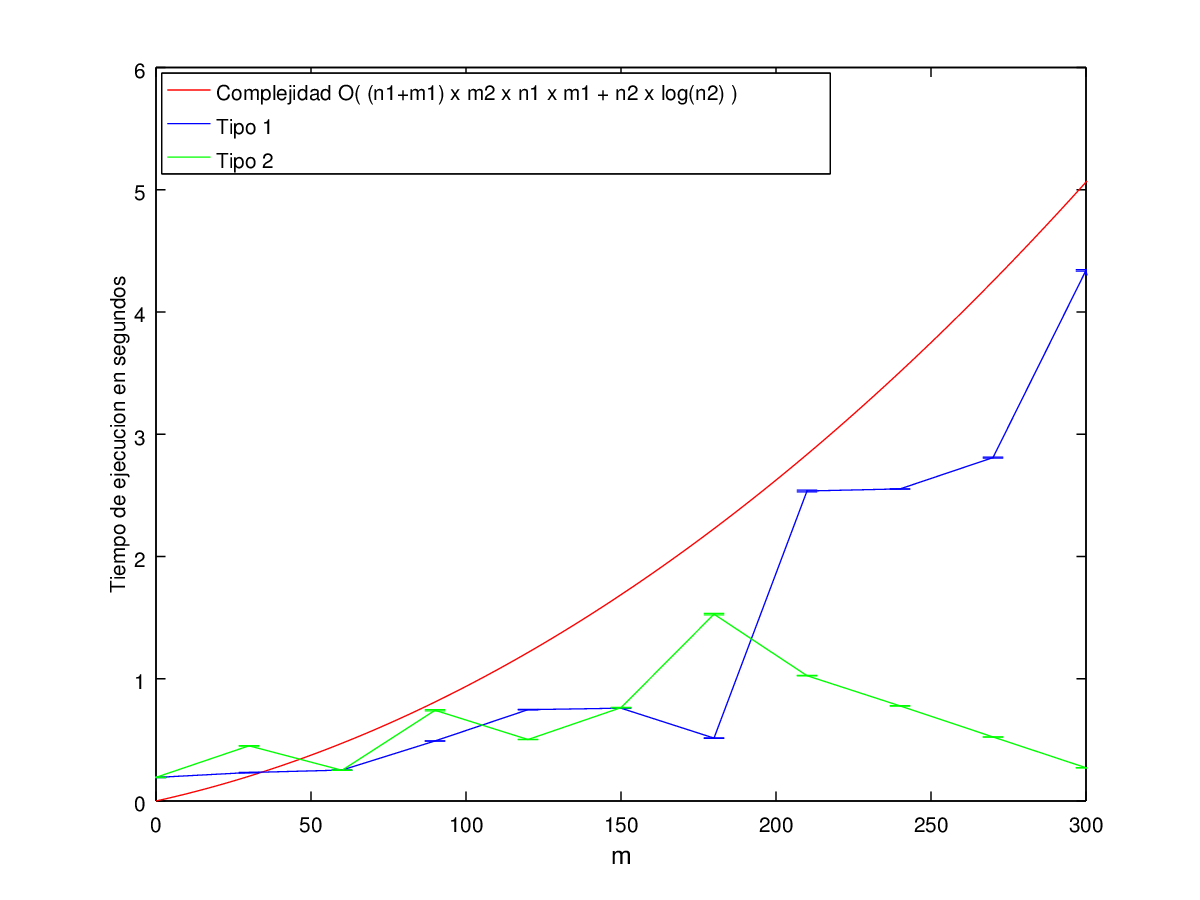
\includegraphics[height=10cm]{graficos/ejercicio5-exp1.png}
       \caption{Experimento 1}
	\end{figure}
    
\subsubsection*{Conclusiones}\;
 Notamos en el gráfico que en ambos casos los tiempos de ejecución de los algoritmos (uno de cada vecindad) están por debajo de la curva de complejidad predicha.\\
 Concluimos que se respeta la complejidad propuesta para el caso de variar el $m_1$.\\
 Adicionalmente notamos que para el algoritmo de vecindad tipo 2, en ciertas instancias de m grande parece tardar menos. Esto podría ser probablemente por un estancamiento rápido en un máximo local (o un casual rápido encuentro de una solución muy buena).\\
 Esta última proposición la volveremos a analizar cuando estudiemos la calidad de las soluciones.
        
        
\subsubsection*{Experimento 2}\;
\noindent Este experimento es similar al anterior, pero ahora se va a variar la cantidad de nodos. Para ello, para cada cantidad de nodos se definirá una función para determinar la cantidad de aristas que tendrá el grafo. \\
\noindent Se tuvieron en cuenta 4 funciones, con el fin de que el grafo obtenido no sea siempre uno especial y de esta forma poder analizar diferentes casos. 
        \begin{itemize}
        \item F1($n_1$) = $n_1$($n_1$-1))/2 = $m_1$ 
        \item F2($n_1$) = $n_1$-1 = $m_1$ 
        \item F3($n_1$) = 3$n_1$
        \item F4($n_1$) = $n_1^{2}$/10
		\end{itemize} 
Para generar los grafos con estas cantidades de aristas y nodos se utilizó el mismo generador que en el experimento anterior.
Este experimento se realiza utilizando primero la vecindad tipo 1 y luego la vecindad tipo 2.
\subsubsection*{Datos de entrada}\;
    \noindent Los valores de $n_1$ tomados fueron desde $10$ hasta $70$ de $5$ en $5$. \\
       Los valores de $n_2$ y $m_2$ fueron $50$ y $200$ respectivamente. El valor de $cuantosVecinosMiro$ fue $20$. Estos valores fueron elegidos de forma arbitraria \\
        Para generar los grafos de forma aleatoria se utilizó el generador-grafo-rapido.cpp que se encuentra en la carpeta src y para correrlo se utilizó el exp2.sh que se encuentra en la carpeta exp/ejercicio5/exp2. \\
        Con el fin de acercarse a los valores reales y descartar posibles falsos resultados, se ejecuta la resolución del problema para cada una de los valores de $n_1$ cinco veces considerando luego el promedio entre los valores obtenidos pero graficando también el desvío estándar (la cantidad de repeticiones a realizar fue elegida arbitrariamente).\; 
\subsubsection*{Resultados}\;

    \begin{figure}[H]
      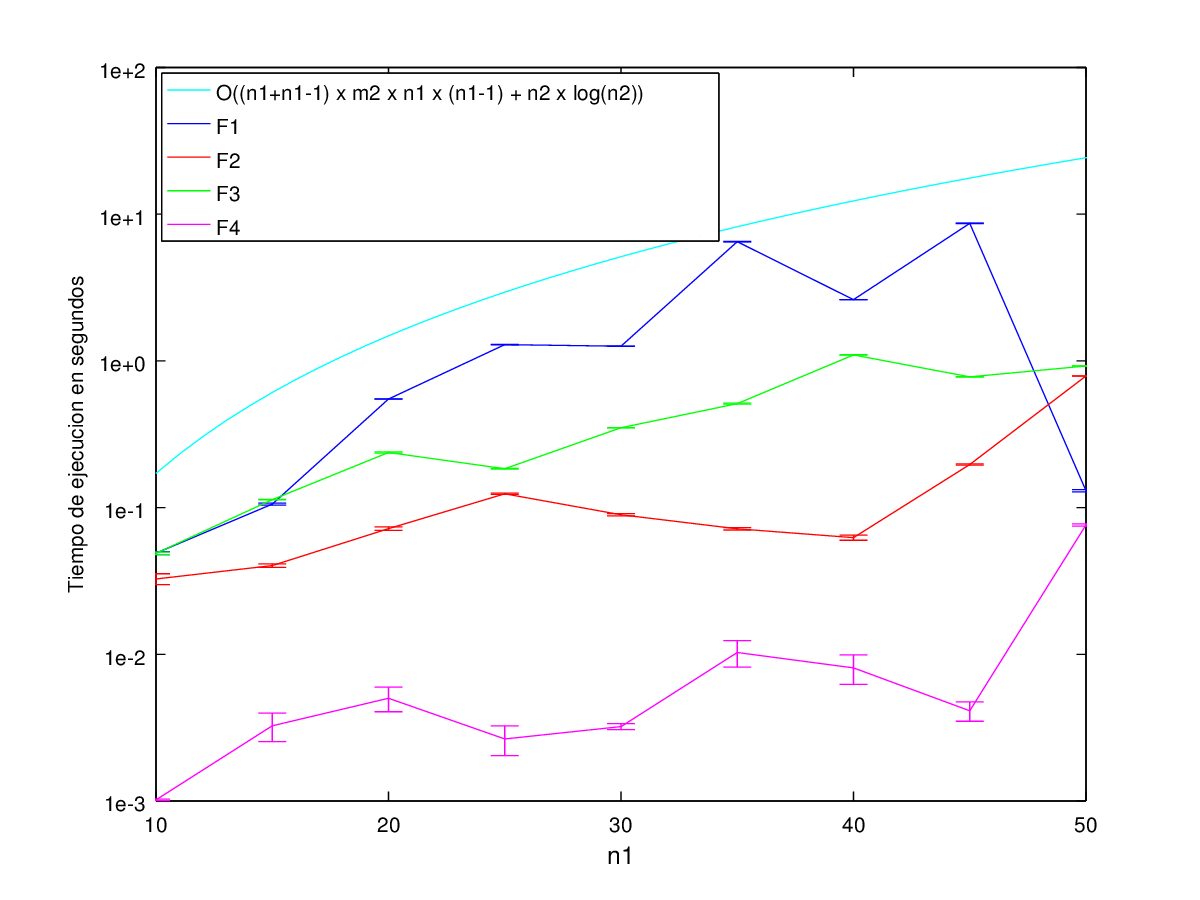
\includegraphics[height=8cm]{graficos/ejercicio5-exp2-tipo1.png}
       \caption{Experimento 2 - Tipo 1}
	\end{figure}
    
        \begin{figure}[H]
      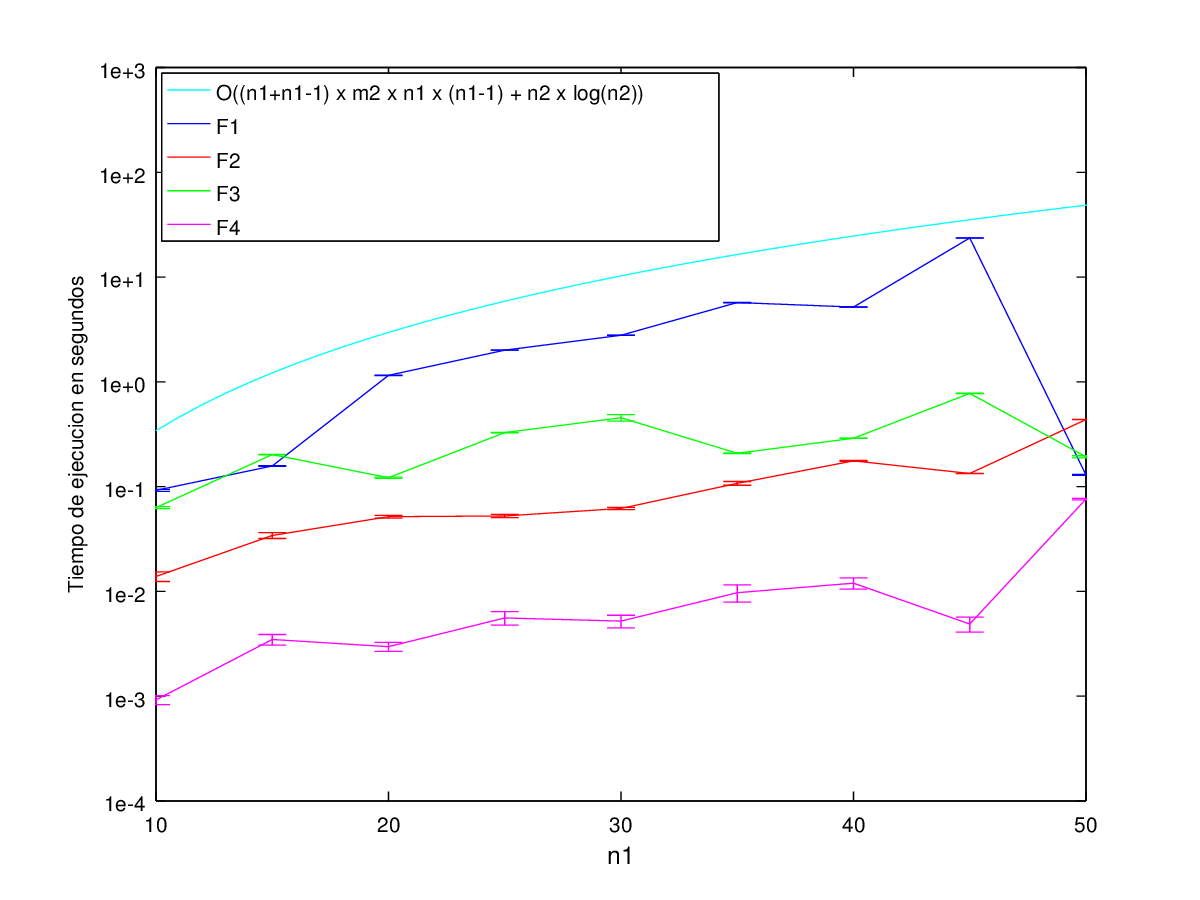
\includegraphics[height=8cm]{graficos/ejercicio5-exp2-tipo2.png}
       \caption{Experimento 2 - Tipo 2}
	\end{figure}
     	
\subsubsection*{Conclusiones}\;
 Se observa en ambos gráficos que se respeta la cota de complejidad prefijada en todos los casos, esto nos lleva a concluir que la cota efectivamente se cumple.\\
 Además puede apreciarse que el desarrollo es similar para ambas vecindades y que ambos algoritmos están dentro del mismo rango en tiempo de cómputo.\\
 También puede apreciarse que los casos de éxito (los casos donde el algoritmo tarda menos) son los mismos, dado que el orden en tiempo de cómputo es el mismo en ambos gráficos, es decir, F1 es el mas lento, seguido de F3, F2 y F4 en ese orden para ambos algoritmos (en ambos grafos es el mismo orden).\\
 Concluimos de este experimento entonces:\\
 \begin{itemize}
\item Se respeta la cota de complejidad propuesta en ambos algoritmos.
\item Los casos de mayor eficiencia en una y en otra vecindad son los mismos.
\end{itemize}
\subsubsection*{Experimento 3}\; 
    El objetivo de este experimento fue extraer conclusiones acerca de la variación en el tiempo de cómputo requerido por el algoritmo para distintos valores de $m$ y $n$ variando los dos grafos al mismo tiempo pero siempre manteniendo $n_1$ igual a $n_2$ y $m_1$ igual a $m_2$. \\
Para generar los grafos con estas cantidades de aristas y nodos se utilizó el mismo generador que en el experimento anterior. 
Este experimento se realiza utilizando primero la vecindad tipo uno y luego la vecindad tipo 2.
        
\subsubsection*{Datos de entrada}\;
    \noindent Los valores de $n$ tomados fueron desde $10$ hasta $70$ de $5$ en $5$. El valor de $cuantosVecinosMiro$ fue $20$. Estos valores fueron elegidos de forma arbitraria. \\
        Para generar los grafos de forma aleatoria se utilizó el generador-grafo-rapido.cpp que se encuentra en la carpeta src y para correrlo se utilizó el exp3.sh que se encuentra en la carpeta exp/ejercicio5/exp3. \\
        Con el fin de acercarse a los valores reales y descartar posibles falsos resultados, se ejecuta la resolución del problema para cada una de los valores de $n$ cinco veces considerando luego el promedio entre los valores obtenidos pero graficando también el desvío estándar (la cantidad de repeticiones a realizar fue elegida arbitrariamente).\; 
\subsubsection*{Resultados}\;

    \begin{figure}[H]
      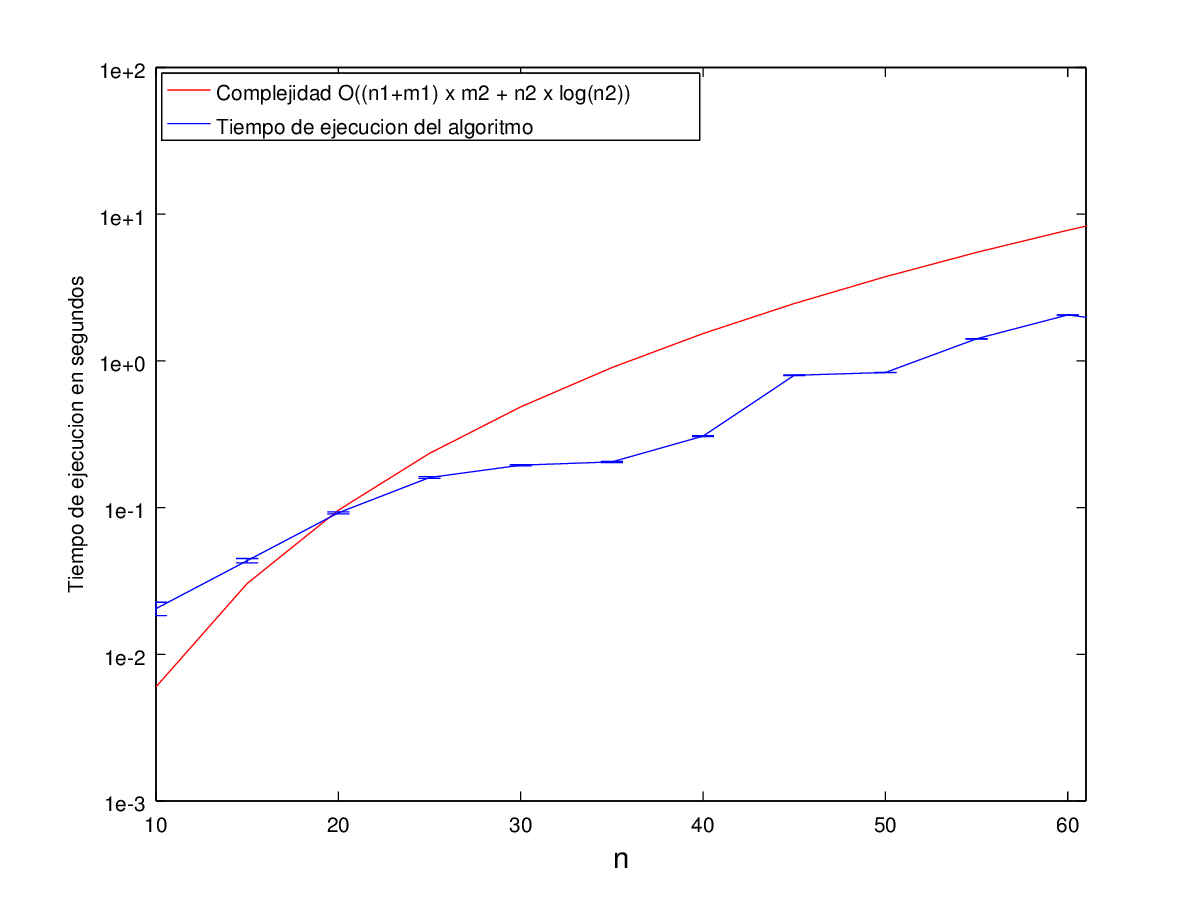
\includegraphics[height=8cm]{graficos/ejercicio5-exp3-tipo1.png}
       \caption{Experimento 3 - Tipo 1}
	\end{figure}
    
        \begin{figure}[H]
      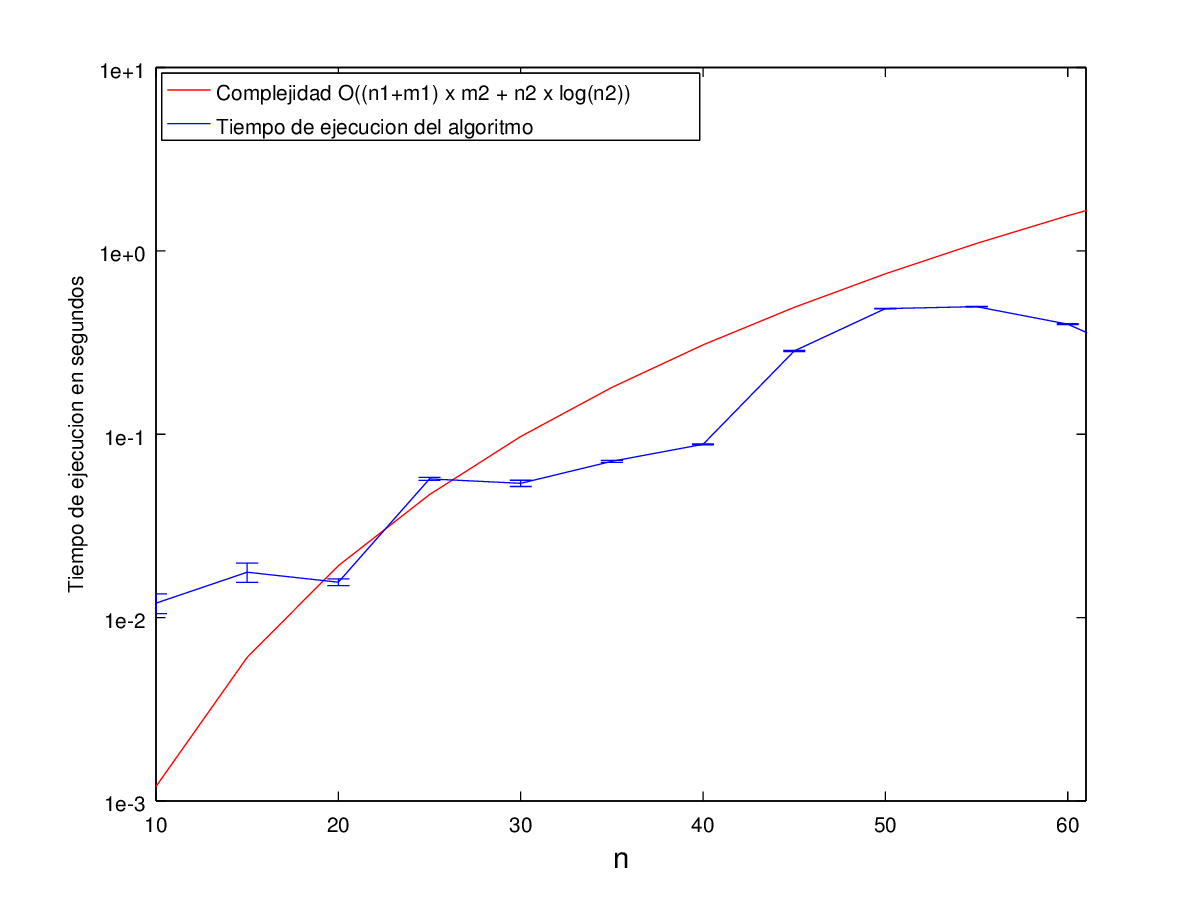
\includegraphics[height=8cm]{graficos/ejercicio5-exp3-tipo2.png}
       \caption{Experimento 3 - Tipo 2}
	\end{figure}


\subsubsection*{Conclusiones}\;
    Se observa y se concluye de este experimento que se respeta la cota de complejidad propuesta en ambos algoritmos, ya que la curva de tiempo de cómputo se sitúa por debajo de la del orden de complejidad.

\subsubsection*{Experimento 4}\;
\noindent El objetivo de este experimento fue comparar los diferentes tipos de vecindades. Para  ello compararemos sobre grafos al azar (variando su tamaño) los tiempos de ejecución por un lado en un gráfico y por otro lado graficaremos la cantidad de aristas de la solución de cada algoritmo (uno de cada vecindad) para así comparar la calidad de las soluciones. \\
Para ello se utiliza el mismo generador que en el experimento 1.\\
Para realizar este experimento se ejecutarán las dos vecindades pasándoles por parámetro de entrada los mismos grafos para poder realizar una comparación más exacta. \\

\subsubsection*{Datos de entrada}\;
    \noindent Los valores de $n_1$ tomados fueron desde $10$ hasta $70$ de $5$ en $5$. \\
       Los valores de $n_2$ y $m_2$ fueron $200$ y $2500$ respectivamente. El valor de $cuantosVecinosMiro$ fue $20$. Estos valores fueron elegidos de forma arbitraria. \\
        Para generar los grafos de forma aleatoria se utilizó el generador-grafo-rapido.cpp que se encuentra en la carpeta src y para correrlo se utilizó el exp4.sh que se encuentra en la carpeta exp/ejercicio5/exp4. \\
        Con el fin de acercarse a los valores reales y descartar posibles falsos resultados, se ejecuta la resolución del problema para cada una de los valores de $n_1$ cinco veces considerando luego el promedio entre los valores obtenidos pero graficando también el desvío estándar (la cantidad de repeticiones a realizar fue elegida arbitrariamente).\; 

\subsubsection*{Resultados}\;

    \begin{figure}[H]
      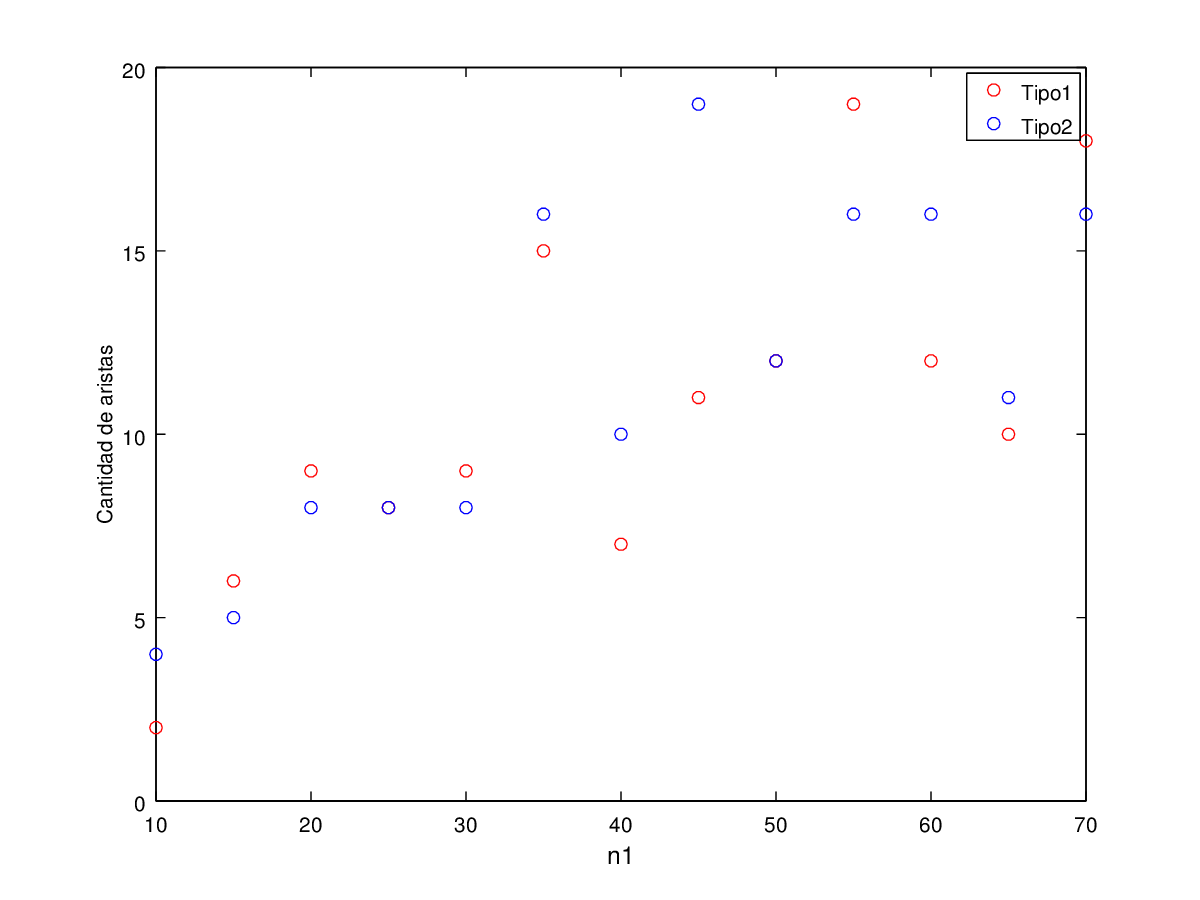
\includegraphics[height=8cm]{graficos/ejercicio5-exp4aristas.png}
       \caption{Experimento 4 - Aristas}
	\end{figure}
    
        \begin{figure}[H]
      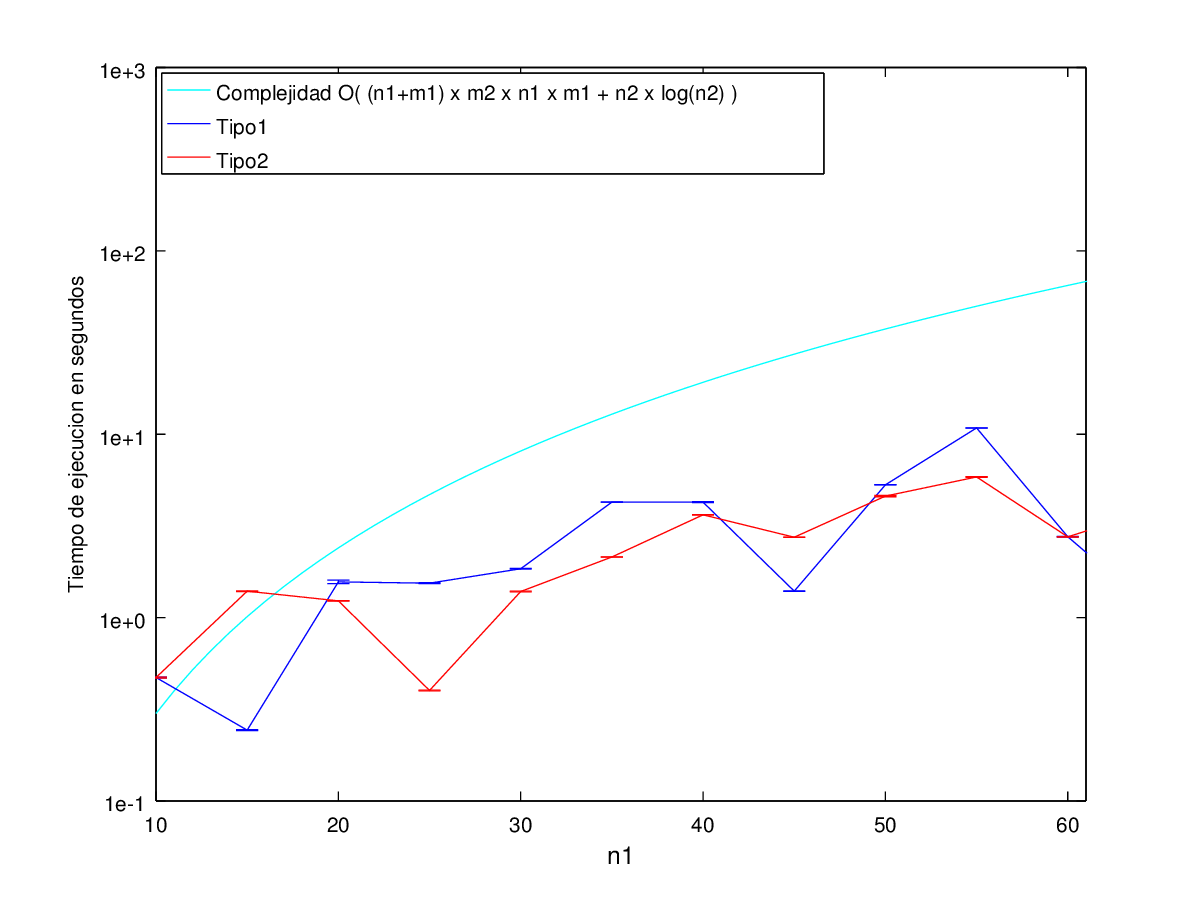
\includegraphics[height=8cm]{graficos/ejercicio5-exp4tiempos.png}
       \caption{Experimento 4 - Tiempos}
	\end{figure}
     	
\subsubsection*{Conclusiones}\;

 \noindent Del primer gráfico (el de la cantidad de aristas por solución), se puede observar una dispersión bastante uniforme, tal vez podría decirse que las vecindades tipo 1 son ligeramente más efectivas en encontrar mejores soluciones (en una gran cantidad de casos), aunque también hay casos en los que se prueba ser mejor elegir vecindades tipo 2.\\
    En los tiempos se observa que ambos cumplen la cota de complejidad predicha, pero no se observa que alguno sea más eficiente que el otro, es decir, son similares en el tiempo de cómputo ambos algoritmos con sus distintas vecindades.\\
    Concluimos entonces que es ligeramente mejor el algoritmo que aplica vecindades tipo 1 ya que es ligeramente mejor en cantidad de aristas y en tiempos, ambos algoritmos son muy similares.